

\section{Which programs can I use to control my detector?}

The complete software package is composed of several programs which can be installed (or locally compiled) depending on the needs:

\begin{itemize}
\item The \textbf{slsDetector shared and static libraries} which are necessary for all user interfaces. \\
  The class slsDetectorUsers can be used as API from your acquisition software (see separate documentation).
\item The \textbf{command line interfaces (sls\_detector\_put, sls\_detector\_get, sls\_detector\_acquire, sls\_detector\_help)}, which are provided to communicate with the detectors using the command line and eventually to the data receiver
\item The \textbf{data receiver (slsReceiver)}, which can be run on a different machine, receives the data from the detector and interfaces to the control software via TCP/IP for defining e.g. the file name, output path and return status and progress of the acquisition
\item The  \textbf{graphical user interface (slsDetectorGUI)} which provides a user friendly way of operating the detectors with online data preview
\item The  \textbf{calibration wizards (energyCalibrationWizard, angularCalibrationWizard)} to analyze the data and produce the energy or angular calibration files
\end{itemize}

\section{How can I control many detectors in parallel or independently?}

For most users the detector will be composed by a single module. Therefore all configurations of the detector will refere to that single entity.

However, for some experiments it is necessary to concatenate the data from several detector controllers, and sometimes (e.g. MYTHEN) each controller can control many modules. This should be transparent to the user since most parameters will be identical for all controllers (e.g. exposure time, energy threshold etc.), except for the configurations specific to the controller (e.g. hardware configuration).\\
In principle it is possible to combine controllers of different type (e.g. MYTHEN, GOTTHARD, EIGER) but the user should then evaluate if it really makes sense to control such different systems in parallel.

In other cases, several SLS detectors will independently acquire data during the same experiment. In this case it will be necessary to be able to seperately control them.

The detectors can be controlled in parallel from several PCs (clients). However it is important the the configurations match on all of the them such that no conflict arise. Eventually a detector can be locked to a specific control PC, still different users interfaces (command line, GUI) can be used in parallel.

A sketch of a possible complex detector configuration is shown in figure~\ref{fig:multidet}

%\section{Detector indexes}

For this reason and index is assigned to each detector. If a single detector is used, as in most cases, the index will be omitted and defaults to 0.\\
To control the other detectors the index cannot be omitted!\\


An index will also be assigned to each controller within a detector. However the user normally will not need to address single controllers, except for the most advanced settings which can be left to configuration files.\\


Finally each module within a controller has an internal index. However in general it is not required that the user is aware of the system architecture and, if needed (rarely), the modules can simply be addressed sequentially starting from controller 0.



\begin{figure}
\caption{Scketch of a possible complex system architecture composed of several detector, each consisting in many controllers eventually controlling several modules.}\label{fig:multidet}
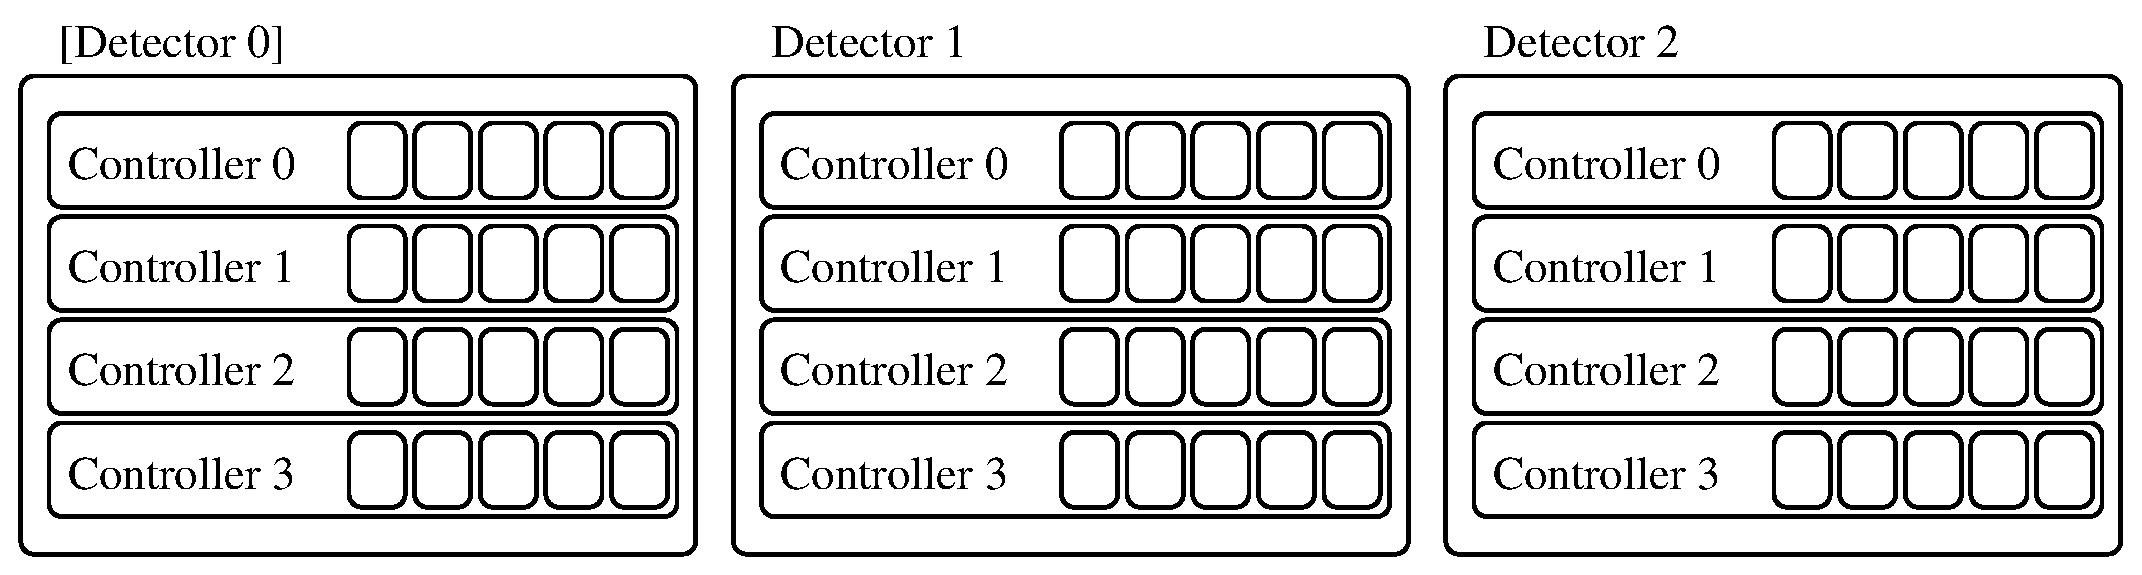
\includegraphics[width=\textwidth]{multi_detector}
\end{figure} 

\subsection{Examples}

For MYTHEN, if one needs to control 6 modules, the system can either be composed by and MCS6 with 6 modules (1 detector, 1 controller, 6 modules), or by 6 MCS1 (1 detector, 6 controller, 1 module each). After apppropriate configuration of the system, the interface to the user will be the same for both systems.

For GOTTHARD, one module corresponds to one controller. A detector will have the smae number of controllers and modules.

For EIGER, one module consists in two controllers. Fo a multi-module system, the number of controllers will increase accordingly, but should be left to a configuration file.

You will need to configure more than one detector, only in case you want to operate several detectors independently.


\section{How can I configure the data receiver?}

For slower acquisitions, the detector will return the data to the control PC over TCP/IP (e.g. MYTHEN).

However, for faster frame rates (e.g. GOTTHARD, EIGER) the controllers will return the data to a data receiver i.e. a process specifically designed to receive the data from the controller over a GBit network and save them to disk. \\
The data receiver can run on any machine (e.g. a file server) accessible by both the control PC and the detector controller, as sketched in figure~\ref{fig:datareceiver}. A data receiver process must be configured for each controller. Normally, to avoid performance loss it is better if different data receivers run on different machines.

\begin{figure}
\caption{Scketch of the communication between the control PC, the detector and the data receiver.}\label{fig:datareceiver}
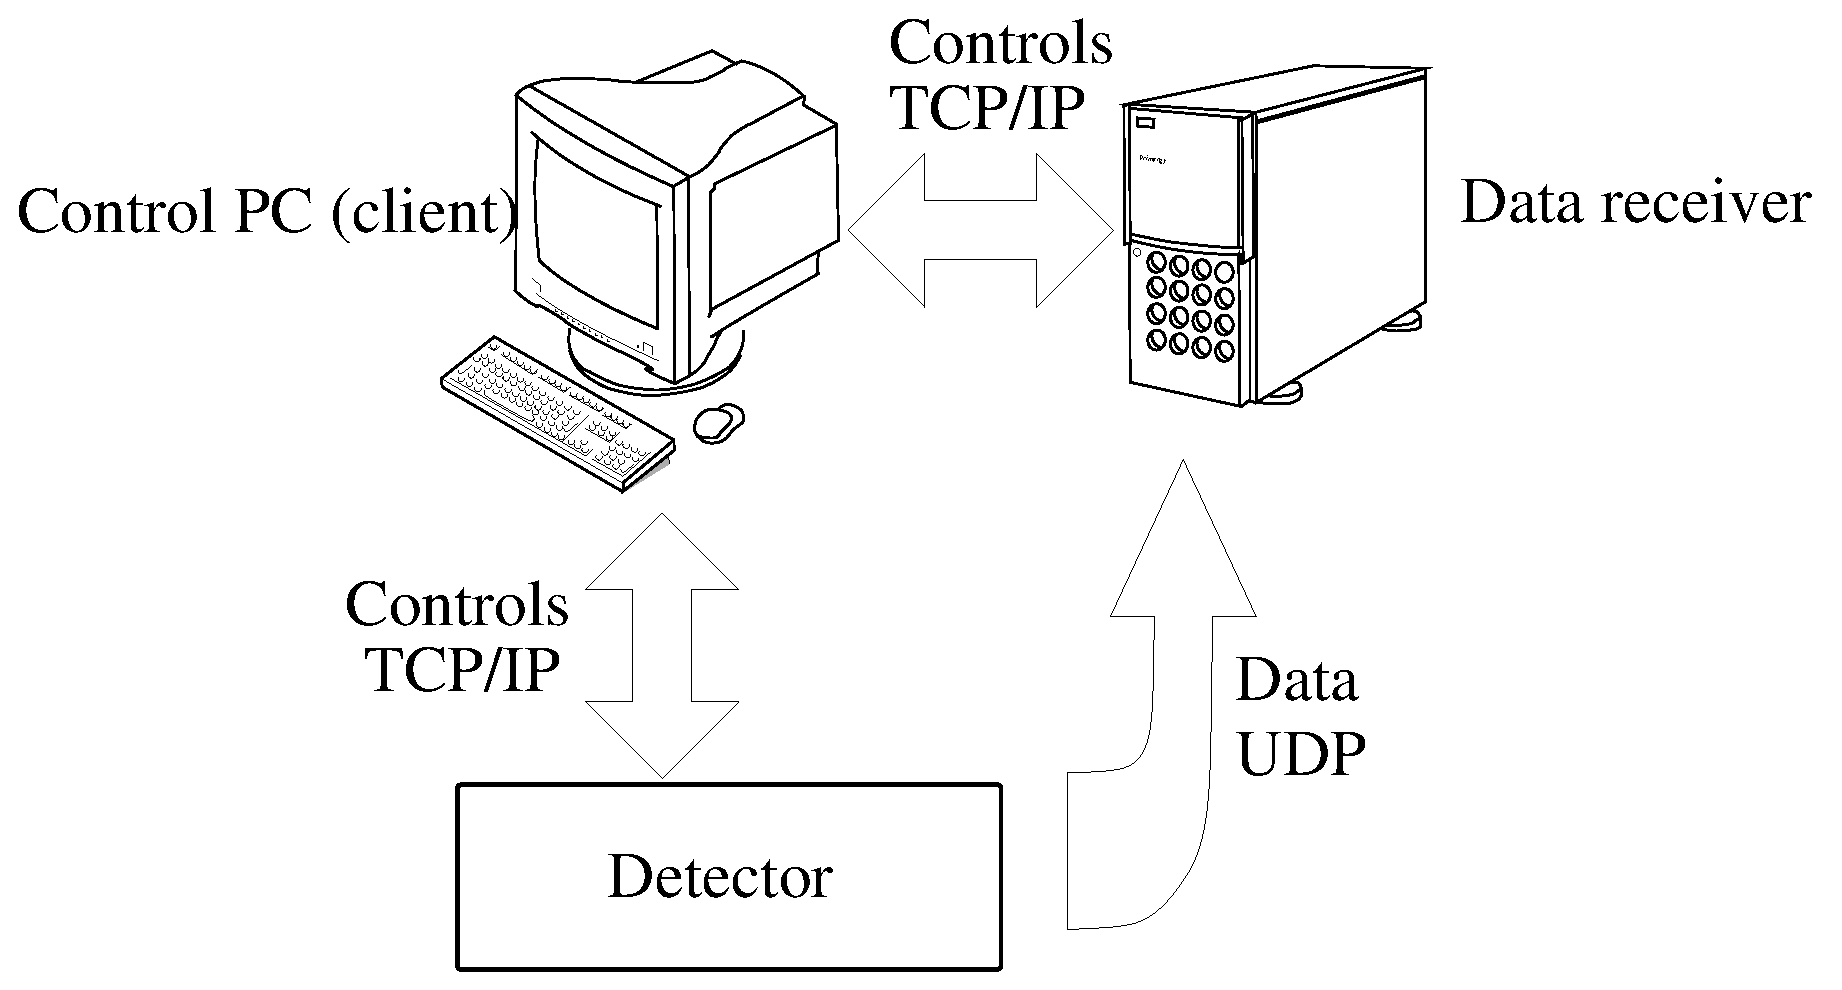
\includegraphics[width=\textwidth]{data_receiver}
\end{figure} 


 
To setup the system, you should configure:
\begin{description}
\item[Client-Detector TCP/IP connection] i.e. for each controller hostname  or IP address  (\textit{hostname}) and communication port (\textit{port}, use default).
\item[Client-Receiver TCP/IP connection] i.e. hostname or IP address of the data receiver (\textit{rx\_hostname}) and communication port (textit{rx\_tcpport}, use default).
\item[Detector-Receiver UDP connection] i.e.  for each controller IP address of the receiver network interface (\textit{rx\_udpip}) and communication port (\textit{rx\_udpport}) used for receiveing the data. By detfault the IP address of the TCP/IP receiver interface will be used also for the UDP conenction. Editing the UDP network interfaces and ports is useful if several controller are sending data to a single receiver (not reccomended to avoid performance loss).\\
A MAC  (\textit{detectormac}) and IP address (\textit{detectorudpip}) should also be assigned to the controller network interface used for the UDP communication, but the default values can normally be used unless firewalls are defined between the detectors and the receiver.
\end{description}
All these configurations are normally left to the configuration file and should not be changed dynamically by the user.

After starting the data receiver process and correctly configuring the client and the detector, this architecture should be completely transparent for the user, except that the output file path must be properly configured from the client for the data receiver machine (easiest is that the disk is mounted for both machines in the same location).\\
The client will take care of communicating with the data receiver and the detector. A feedback about the progress of the acquisition and a preview of the data being acquired can also be obtained by the client from the data receiver.



\section{What are settings and calibration files for?} \label{sec:trimdir}

The analog characteristics of the detector have to be initialized in order to define the noise and the dynamic range which need to be used for the measurements. These parameters have a different meaning for analog or digital detectors, but in both cases some predefined voltage levels and current (we call them \textit{settings}) must be laoded to the detector. Moreover, there are some parameters that are custom to single detectors or modules (e.g. the trimbits). All these settings are stored in some settings file, which are organized in a \textit{settingsdir} with a definite architecture, where the software will look for the files to load to the detector whaen changing its settings.

In addition to that, in a single photon counting detector the threshold is set as a voltage level for the comparator, but for the user it is useful to have a direct conversion to the energy level. For this, after a proper calibration of the detector (see specific documentation) calibration file are generated in order to convert threshold in volts to keV. Also in this case the directory \textit{caldir} where the calibration files are stored must be defined ad organized with a proper architecture, suche that the software can find the calibration coefficients for settings the threshold.\\
Normally \textit{settingsdir} and \textit{caldir} can be the same, but have been left separate for flexibility.

The \textit{settingsdir} and \textit{caldir} should be properly configured for your detector either in a configuration file (for use with text clients, GUI or API) or dynamically (works only for the text clients).

In the following, the architecture of the \textit{settingsdir} and \textit{caldir} is described for the different detectors.

\subsection{MYTHEN}
For mythen, an example of \textit{settingsdir} and \textit{caldir} is  given in the software package by the directory \verb=trimdir=. 
Since these directories are customized by producing trimbit files and calibration for each detector, make sure not to overwrite yours every time you upgrade the software.

\textit{settingsdir} should contain three subdirectories \verb=standard=,  \verb=fast= and  \verb=highgain= containing respectively the trimfiles \verb=standard.trim=,  \verb=fast.trim= and  \verb=highgain.trim= which contain the correct voltage settings for the detector although all the individual channel thresholds set to 0. The original files contained in the package should be used, infact in case of error the detector would not recognize the correct settings.\\
The default trimbit files for each file will be stored in the directory according to the settings with the name \verb=noise.snxxx= where \verb=xxx= is the module serial number.\\

\textit{caldir} should contain three subdirectories \verb=standard=,  \verb=fast= and  \verb=highgain= containing respectively the trimfiles \verb=standard.cal=,  \verb=fast.cal= and  \verb=highgain.cal= which contain an average calibration of the modules for the diffrent settings. However this can different from the correct one for each individual module even of several kev and therefore it is very important to perform an energy calibration on a module basis.\\
The default calibration files for each file will be stored in the directory according to the settings with the name \verb=calibration.snxxx= where \verb=xxx= is the module serial number.


\subsection{GOTTHARD}
A \textit{settingsdir} should be configured, as the directory  \verb=settings= in this software package.\\
It must contain the subdirectories \verb=dynamicgain=, \verb=gain1=,  \verb=gain2=,  \verb=gain3=,  \verb=highgain=,  \verb=lowgain=,  \verb=mediumgain=, and   \verb=veryhighgain= in order to properly configure the GOTTHARD detector using the various gain settings.


\section{How should a configuration file look like?}

A configuration file is a list of command necessary to properly configure your detector systems, with default valuee for some parameters and other settings that the users should normally not change dinamically.
For this reason most of the commands present in the configuration file cannot be modified when using the API.\\
The syntax of the configuration file is exactly the same as in the comman line interface, therefore you can refere to that documentation to edit the files.\\
The configuration files look different for the different detector types. Examples of configuration files can be found in the examples directory.

\section{What is the meaning of the file name?}
The final file name will be: \\
\textit{outdir/prefix}\verb=[_d=$d$\verb=][_S=\textit{v0}\verb=][_s=\textit{v1}\verb=][_p=\textit{p}\verb=][_f=\textit{f}\verb=]_=\textit{i}\verb=.=\textit{ext}\\
where: \\
\textit{outdir} is the output directory path;\\
\textit{prefix} is the chosen prefix for the file name;\\
\textit{d} is the detector index, in case of data receiver and more than one detector;\\
\textit{v0} is the scan0 variable with the desired precision, if scan0 is enabled;\\
\textit{v1} is the scan1 variable with the desired precision, if scan1 is enabled;\\
\textit{p} is the position index, if different positions are configured;\\
\textit{f} is the frame index of the first frame stored in the file, if many frames and triggers are configured;\\
\textit{i} is the file index;\\
\textit{ext} is the file extension e.g. \textit{.raw} for MYTHEN raw data, \textit{.dat} for MYTHEN processed data.

\section{Which is the sequence of the acquisition flow?}

The software gives the  possibility to setup several loops, actions and scan utilities which are then handled during the acquisition. 
The software will also take care to generate the file names  and increment the indexes accordingly.\\

Figure~\ref{eq:acqflow} shows in which sequence the various scripts and loops are executed when calling the acquire command. The loops are drawn using the $\Updownarrow$ symbol, while the scripts using the  $\Rightarrow$.


\begin{displaymath} \label{eq:acqflow}
%%%%%%%%%%%%%%%%%%%%%8
  \textrm{\textbf{MEASUREMENTS}} \\
 \left\Updownarrow \,
    \begin{array}{l} \\
  %   \textrm{Measurement loop} \\
  %   \\
%%%%%%%%%%%%%%%%%%%%%7
    % \left[ 
   %  \,
           \begin{array}{l} %\\
        	  \Rightarrow  \,  \textrm{Start script} \\
	   \\
%%%%%%%%%%%%%%%%%%%%%6
                    \textrm{\textbf{SCAN0}}
           \left\Updownarrow 
     \,
	          \begin{array}{l} \\
                 	  \Rightarrow \,  \textrm{Scan0 script} \\
           %        \textrm{Scan 0 level} \\
		   \\
%%%%%%%%%%%%%%%%%%%%%5
     
                    \textrm{\textbf{SCAN1}}      \left\Updownarrow  
     \,
	          \begin{array}{l} \\
                %   \textrm{Scan 1 level} \\
		 %  \\
%%%%%%%%%%%%%%%%%%%%%4
          % \left[  
   %  \,
	          \begin{array}{l} %\\
                 	  \Rightarrow \,  \textrm{Scan1 script} \\
                 	  \Rightarrow \,  \textrm{Script before} \\
		   \\
%%%%%%%%%%%%%%%%%%%%%3
     %      \left\Updownarrow       \,
	          \begin{array}{l} \\
                    \textrm{\textbf{POSITIONS}} \left\Updownarrow  \,	  
%%%%%%%%%%%%%%%%%%%%%2
	          \begin{array}{l} \\
             	  \Rightarrow \,     \textrm{Header before script} \\
		   \\
%%%%%%%%%%%%%%%%%%%%%1
       
                   \textrm{\textbf{CYCLES}}     \left\Updownarrow  \,
	          \begin{array}{l} \\
		  \\
%%%%%%%%%%%%%%%%%%%%%0
		  \textrm{\textbf{FRAMES}}    \left\Updownarrow  \right. \\ 
		  \\
%%%%%%%%%%%%%%%%%%%%%%%%%%0
		  \\
		  \end{array}
		  \right. \\ 
		  \\
%%%%%%%%%%%%%%%%%%%%%%%%%%1
        	  \Rightarrow \,  \textrm{Header after script}\\
		  \\
		  \end{array}
		  \right. \\ 
%%%%%%%%%%%%%%%%%%%%%%%%%%2
\\
\\
\\
           \end{array}
%	   \right. I see the digitest works fine, and this is good news.

		  \\ 
	 %  \\
%%%%%%%%%%%%%%%%%%%%%%%%%%3
	  \Rightarrow \, \textrm{Script after} \\
%\\
                   \end{array}
	  % \right. \\ 
	   \\
%%%%%%%%%%%%%%%%%%%%%%%%%%4
\\
                   \end{array}
	   \right. \\ 
\\
	   \\
%%%%%%%%%%%%%%%%%%%%%%%%5
\\
                   \end{array} 
	   \right. \\
	   \\
%%%%%%%%%%%%%%%%%%%%%%%%6
	  \Rightarrow	\,   \textrm{Stop script} \\
\\
            \end{array} 
 %     \right. \\
 %     \\
%%%%%%%%%%%%%%%%%%%%%%%%7
\\
      \end{array}  
\right. 
%%%%%%%%%%%%%%%%%%%%%%%%8
\end{displaymath}


If you prefere to handle the acquisition from your acquisition enviroment, simply leave al scripts and scans disabled and call the acquition from your acquisition enviroment. \\
Only the frames and triggers loops are defined in firmware and guarantee a precise timing of the acquisition which cannot replaced by any other method (you can synchronize to your beamline by hardware connection of the IO signals as described in~\ref{sec:timing}).

Hereafter a description of the meaning of the various loops:
\begin{description}
\item[Measurement loop] executes offline several times the entire sequence of the acquisition. At the end of each measurement the \textit{file index} is incremented.

\item[Scan 0 loop]
  is a high level scan loop which can be used e.g to loop on an enviroment variable (temperature, humidity...) or even to change sample.\\
 The list of steps or range of the \textit{scan0 variable} must be set as scan0steps or scan0range. For small steps of the scan variable, avoid overwriting of the files specifying all the necessary digits in the filename by properly setting the precision with scan0prec.

\item[Scan 1 loop]
  is a low level scan loop which can be used e.g to loop on an enviroment variable (temperature, humidity...) or to move the sample in case of radiation damage.\\
 The list of steps or range of the \textit{scan1 variable} must be set as scan1steps or scan1range. For small steps of the scan variable, avoid overwriting of the files specifying all the necessary digits in the filename by properly setting the precision with scan1prec.

\item[Position loop]
 The detector is moved in the angular positions specified by the positions command.\\
 The command for moving the detector should be defined as described in~\ref{sec:usersFunc}.\\
 All data acquired during a position loop will be merged together, unless the number of positions is set to 0. In this case single frames will be converted to angle without merging.\\
 Avoid using the position loop together with many frames/triggers.

\item[Triggers loop] is executed in real time and defines e.g. the number of triggers that will be accepted. The total number of images will be given by frames times triggers.

\item[Frames loop] is executed in real time and defines e.g. the images acquired per trigger. The total number of images will be given by frames times triggers.
\end{description}

Executing a script simply consists in a system call with the arguments specified below. The various scripts are executed only if they are enabled and different than \textit{none}. \\
The scripts must be executable and the capability of parsing the arguments passed by the acquition program is left to the user writing the scripts. some example scripts writte in awk can be found in the examples directory.\\
Hereafter a short description of how the scripts are called and with which options:
\begin{description}

\item[Start script]
     is executed at the very beginning of the measurement and can be used e.g. to initialize all the devices needed for the acquisition or open the beamline valves. The script is executed as:\\
      script  nrun=i par=p\\
      where i is the  \textit{file index} and p is the \textit{start script parameter}.

\item[Scan0 script]
  There are a few predefined scan modes i.e. \textit{threshold} changing the detector threshold in DAC units, \textit{energy} chaning the calibrated detector threshold in eV, \textit{trimbits} chaning the trimbits of the detector (advanced: do not use) and \textit{position} changing the detector position (if the motor movement is correctly setup as described in~\ref{sec:usersFunc}). Otherwise the scan0script is executed as:\\
 script nrun=i fn=fn var=v par=p\\
  where i is the  \textit{file index}, fn is the \textit{file name}, v is the value of the \textit{scan0 variable} at the present step of the scan0 loop and  p is the \textit{scan 0 script parameter}.

\item[Scan1 script]
  There are a few predefined scan modes i.e. \textit{threshold} changing the detector threshold in DAC units, \textit{energy} chaning the calibrated detector threshold in eV, \textit{trimbits} chaning the trimbits of the detector (advanced: do not use) and \textit{position} changing the detector position (if the motor movement is correctly setup as described in~\ref{sec:usersFunc}). Otherwise the scan1script is executed as:\\
 script nrun=i fn=fn var=v par=p\\
  where i is the  \textit{file index}, fn is the \textit{file name}, v is the value of the \textit{scan1 variable} at the present step of the scan1 loop and  p is the \textit{scan 1 script parameter}.

\item[Script before]
  is called just before the beginning of the data taking and can be used e.g. to open the shutter.
  The script is executed as:\\
  script nrun=i fn=fn par=p sv0=v0 sv1=v1 p0=p0 p1=p1 \\
  where i is the  \textit{file index}, fn is the \textit{file name}, p is the \textit{script before parameter}, v0 and v1 are the  values of the \textit{scan0 and scan1 variables} at the present step of the scan loops and  p0 and p1 are the \textit{scan0 and scan1 script parameters}.
  

\item[Header before script]
    is called before every step of the data taking (i.e. for each position, but at the beginning of the frames train if several acquisition have been programmed in real time) and can e.g. be used to dump the exact settings of the detector and beamline to reproduce or analyze the data offline.
    The script is executed as:\\
    script nrun=i fn=fn par=p\\
    where i is the  \textit{file index}, fn is the \textit{file name}, and p is the \textit{header before parameter}.

\item[Header after script]
    is called after every step of the data taking (i.e. for each position, but at the end of the frames train if several acquisition have been programmed in real time) and can e.g. be used to dump the exact settings of the detector and beamline to reproduce or analyze the data offline.
    The script is executed as:\\
    script nrun=i fn=fn par=p\\
    where i is the  \textit{file index}, fn is the \textit{file name}, and p is the \textit{header after parameter}.

\item[Script after] 
  is called just after the end of the data taking and can be used e.g. to close the shutter.
  The script is executed as:\\
  script nrun=i fn=fn par=p sv0=v0 sv1=v1 p0=p0 p1=p1 \\
  where i is the  \textit{file index}, fn is the \textit{file name}, p is the \textit{script after parameter}, v0 and v1 are the  values of the \textit{scan0 and scan1 variables} at the present step of the scan loops and  p0 and p1 are the \textit{scan0 and scan1 script parameters}.
  
\item[Stop script]
     is executed at the very end of the measurement and can be used e.g. to switch off all devices. The script is executed as:\\
      script  nrun=i par=p\\
      where i si the \textit{file index} and p is the \textit{stop script parameter}.

\end{description}






\section{How can I synchronize my detector with the experiment?}\label{sec:timing}

The timing of the detector is always defined by an active detection time followed by a dead time during which the detector is read out. This read out time as a fixed duration depending on the detector type and its configuration (e.g. dynamic range) which limits the maximum frame rate achievable.\\
In the following is a list of the main parameters involved in the acquisition timing:
\begin{description}
\item[Exposure time] is the time during which the detector is detecting X-rays for each image (ignored is the timing mode is \textit{gating}).
\item[Period] is the period of the images acquired. If it is shorter than the exposure time plus readout time, it will be ignored.
\item[Delay after trigger] can be set as a delay between the trigger signal and the start of the detection time. 
\item[Number of gates] is used only in \textit{gating} mode and is the number of times that the gate is toggled before the detector is read out. Useful for stroboscopic measurements with gate period shorter than the minim acquisition period of the detector, otherwise can be left to 1.
\item[Number of frames] is the number of images to be acquired per cycle. Frames and triggers have the same meaning except in trigger mode, when frames means the number of images per trigger. The total number of images is frames time triggers.
\item[Number of triggers] is the number of times that the frames are acquired. Frames and triggers have the same meaning except in trigger mode, when triggers means the number of triggers that will be accepted. The total number of images is frames time triggers.
\item[Number of probes] is used in stoboscopic measurements when the period is longer than the minimum acquisition period, but shorter than the frame rate.\\
In this case the data can be summed in firmware. \\
Currently it is implemented for Mythen only. If probes is set to 0, works normallyreturning an image for each readout, otherwise set number of triggers to 1. The maximum number of probes that can be set is 3. The detector will return a number of image equal to the number of probes, where all frames are going to be accumulated. The total number of readouts is number of frames time probes and for  probes=1 the detector will return one image where all frames have been summed, for  probes=2 two images where every second frame has been summed (each image accumulates the number of frames), for probes=3 three images where every third image has been summed (each image accumulates the number of frames).\\
The returned images will always have 32~bit dynamic range, while the dynamic range if the detector defines the bit depth of the counters in rder to limit the readout time, if necessary.\\
The probes counter waorks also in trigger and gating modes.
\end{description}





\begin{figure}
\begin{center}
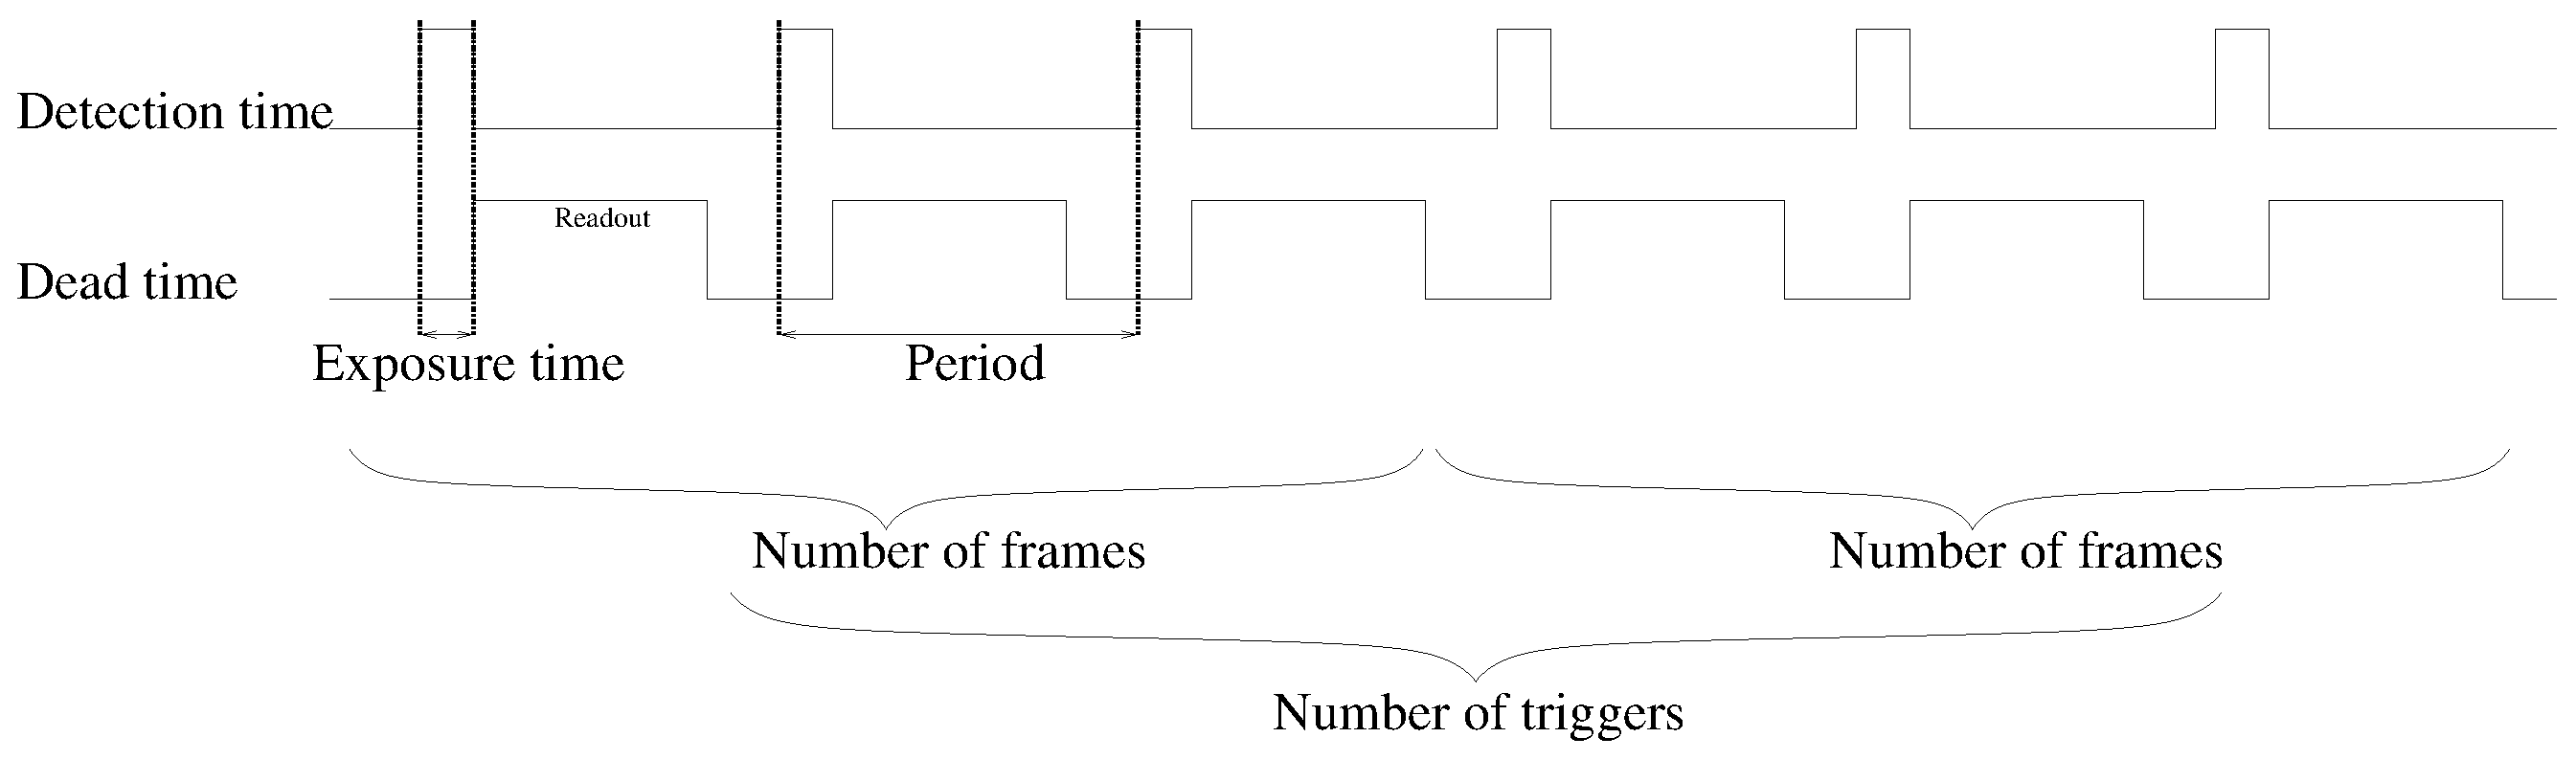
\includegraphics[width=\textwidth]{images/normal_acquisition.eps}
\end{center}
\caption{Auto timing: the detection time is defined by the exposure time and the period by period (if longer than exposure time plus readout time). The total number of images is frames (in the example 3) times triggers (in the example 2), and in this case there is no difference between the acquisition of the two.}\label{fig:autotiming}
\end{figure}

\begin{figure}
\begin{center}
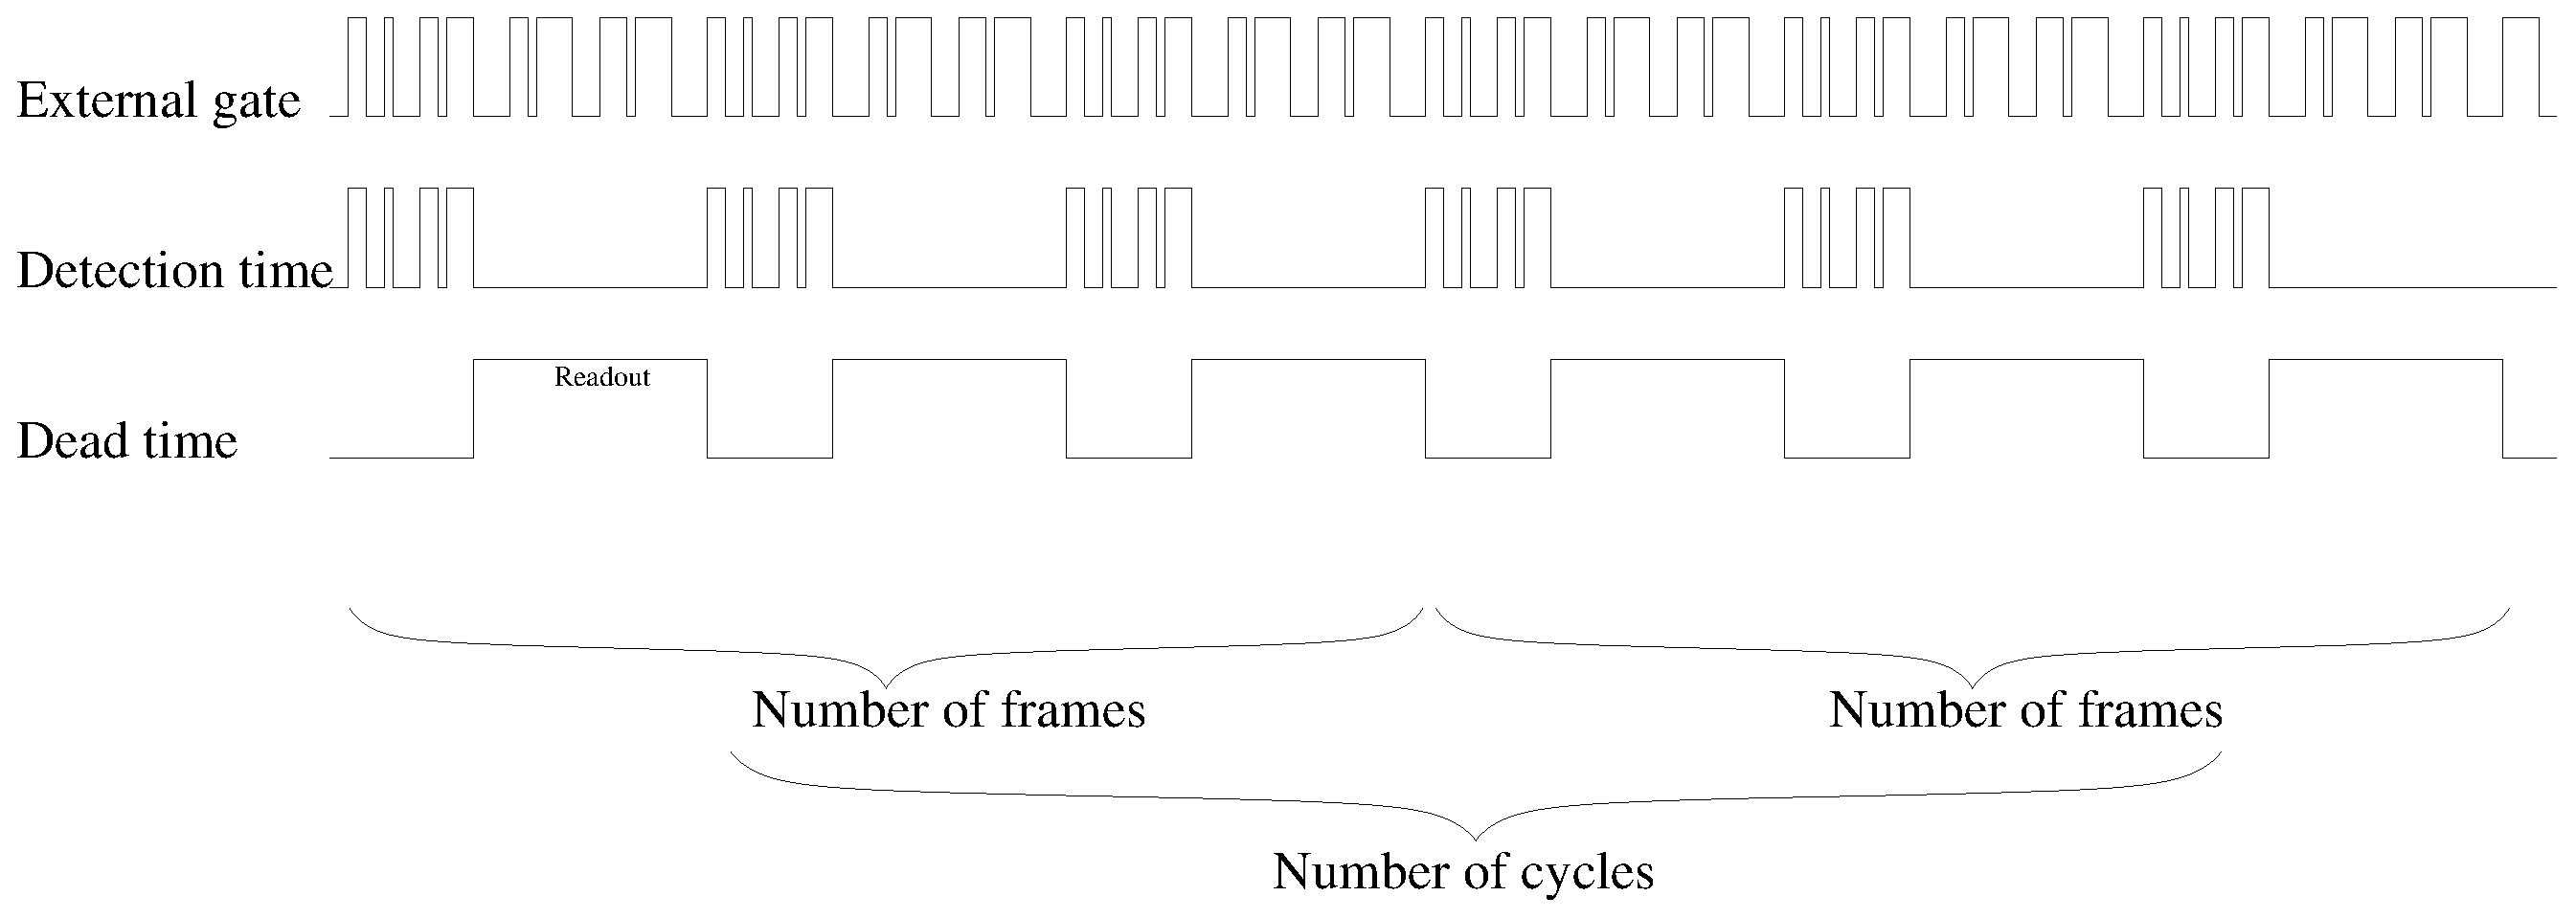
\includegraphics[width=\textwidth]{images/gated_acquisition.eps}
\end{center}
\caption{Gating mode: the detector acquires for a number of gates define by the  user (in this case 4) before being read out, independently on the timing of the gates. The detector remains insensitive during the readout time and then starts being active again. External gates given during the readout time are ignored. The total number of images is frames (in the example 3) times triggers (in the example 2), and in this case there is no difference between the acquisition of the two. The polarity of the external gate signal can be defined by the user through the \textit{external signal flag} (in the example active high).}\label{fig:gating}
\end{figure}



\begin{figure}
\begin{center}
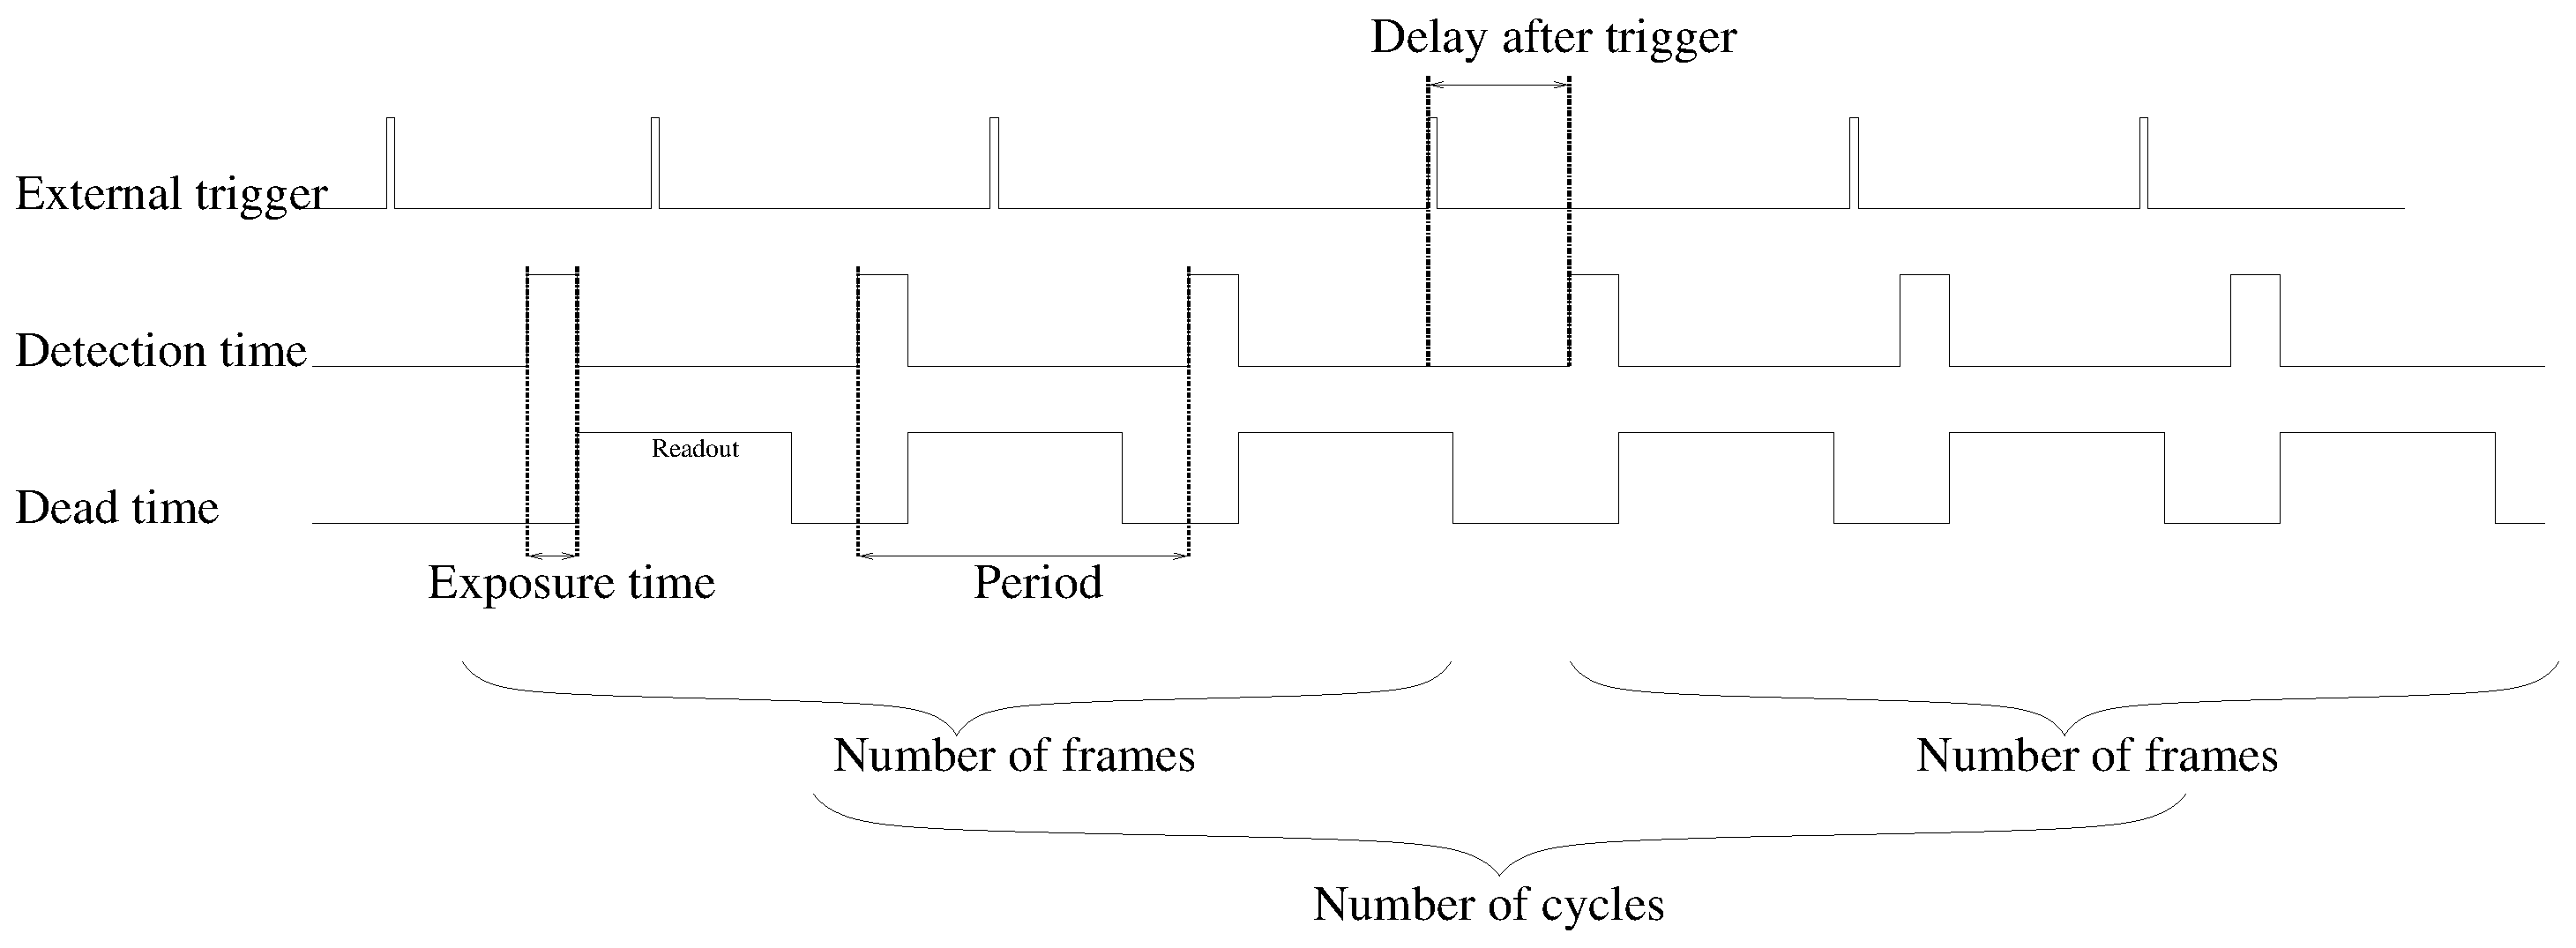
\includegraphics[width=\textwidth]{images/trigger_acquisition.eps}
\end{center}
\caption{Trigger mode: the external trigger signal defines the start of the beginning of the acquisition, which starts after the delay set by the user. For each trigger, the number of frames is acquired (in the example 3) and all trigger signals ignored. The number of trigger accepted is given by the number of triggers (in the example 2). The polarity of the external trigger signal can be defined by the user through the \textit{external signal flag} (in the example rising edge).}\label{fig:trig}
\end{figure}


\begin{figure}
\begin{center}
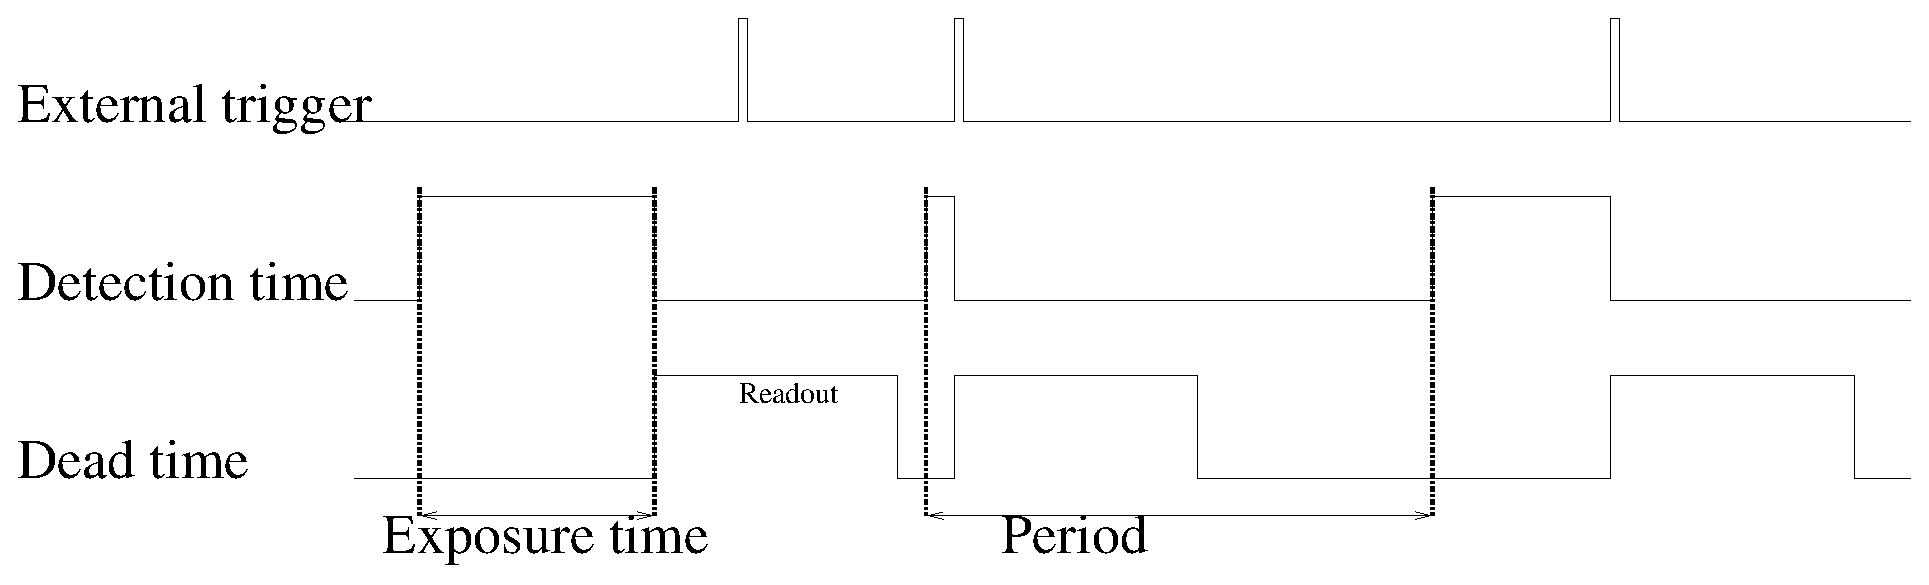
\includegraphics[width=\textwidth]{images/ro_trigger_acquisition.eps}
\end{center}
\caption{Read Out Trigger mode: the external trigger signal defines the beginning of the readout. The exposure time works as a time out for the waiting time for the trigger signal. The number of trigger accepted is given by the number of triggers (in the example 3) and it does not make sense to program more than one frame. The polarity of the external trigger signal can be defined by the user through the \textit{external signal flag} (in the example rising edge).}\label{fig:trig}
\end{figure}


\section{How can several controllers be synchronized?} \label{sec:sync}
If you are not performing time resolved measurements, you will probably not need any synchronization of the controllers: they will be started sequentially by the software and their acquisition will have a jitter of a few ms. \\
In the case you need a precise synchronization, on the other hand, hardware connection is required between the controllers through the external IO signals. The external signals used for this synchronization should be configured as \textit{sync} with the \textit{extsig} command. \\
In this case a \textit{master} controller should be defined for the acquisition which will the send the synchronization signal to the other controllers, while the other controllers will use them as inputs.\\
The type of synchronization can be\textit{gating} or \textit{trigger} depending if the synchronization signal will gate the slave detectors or trigegr the beginning of the acquisition. There are no particular reasons to chose one or the other method, except if the user finds out that one is more stable than the other.\\
Normally the configuration of the synchronization is configured inside the configuration file and should not be changed dynamically by the user.\\

After the configuration, the synchronization of the controllers will be completely transparent for the user, who will simply have to setup the timing parameters of the detector as a whole.

\section{How can the detector movement and position and I0 readout be customized for my beamline?} \label{sec:usersFunc}

The easiest way to allow the software to perform all the necessary normalization and angular conversion steps, is enable it to move your detector and read the encoder position and the value of the ionization chamber.\\
These functions are defines as callbacks and can be redifined by registering your own functions. This is normally a good method if you use the API or are willing to write your main client program.\\
Otherwise the simpleast way is to edit the file\\ 
\verb=slsDetectorSoftware/usersFunctions/usersFunctions.cpp= \\
where the default functions performing these actions are implemented and modify them to interface with your beamline hardware. The functions are written in C and are very simple to implement for anyone with some programming knowledge.\\
A simple high-level solution in case you need to maintain the software for several beamlines and don't want to recompile for all of them is to call external scripts.


\section{In which data format are written the data?} \label{sec:dataFormat}

For MYTHEN the data are writen in ASCII fomat, one file per frame, in columns, either channel number - counts for the \textit{.raw} files or angle (or channel number)-counts-error for the \textit{.dat} files.

For the other detectors the files are written in binary format, and must be decoded depending on the detector.

\subsection{GOTTHARD}
Each file contains 100 frames.
\begin{description}
\item[Normal mode]
Each frame is split into 2 packets of 1286 bytes each, where actual data is 1280 bytes each. Both the packets (incl header and footer) are written one after the other into the file.

Representation of each packet:
\begin{itemize}
\item
The first 4 bytes represents a number from which, the frame number and packet number can be derived.
If the number was 108601, increment it by 1 to get 108602.\\
Then this $(108602\&0xFFFFFFFE)>>1 = 54301$ is the frame number
and  $(108602\&0x1) =0$ is the packet number.\\
0 is the packet on the left and 1 is the packet on the right.\\
On a side note, when you use the data call back, we also give you the derived frame number as an argument.

\item Data of 1280 bytes. 16 bits per pixel.

\item  2 bytes of insignificant footer.
\end{itemize}

\item[Short Frame Mode]
One Frame has only one packet of 518 bytes, where actual data is 512 bytes.
\begin{itemize}
\item   first 4 bytes is the frame number. There is no packet number or increment required herecompared to the normal mode.
\item   Data of 512 bytes.
\item   2 bytes of insignificant footer.
\end{itemize}

\end{description}

\subsection{EIGER}

\subsection{JUNGFRAU}
